\subsection{Projects Module}
\label{sec:mobile-projects}

\textbf{Purpose:}
Provides a centralized interface for managing workflow projects. The Projects module enables users to browse their workflow projects, create new ones, import existing workflows, and control workflow execution directly from the mobile application.

\vspace{0.2cm}
\noindent\textbf{Main Features}

\begin{itemize}
    \item Browse Projects
    \item Search Projects
    \item Create New Project
    \item Import Existing Workflow
    \item Deploy and Stop Workflows
\end{itemize}

%%%%%%%%%%%%%%%%%%%%%%%%%%%%%%%%%%%%%%%%%%%%%%%%%%%%%%%%%%%%

\subsubsection{Projects Screen}

\textbf{Purpose:}
Displays all workflow projects associated with the authenticated user while providing quick access to workflow management operations.

\begin{figure}[H]
    \centering
    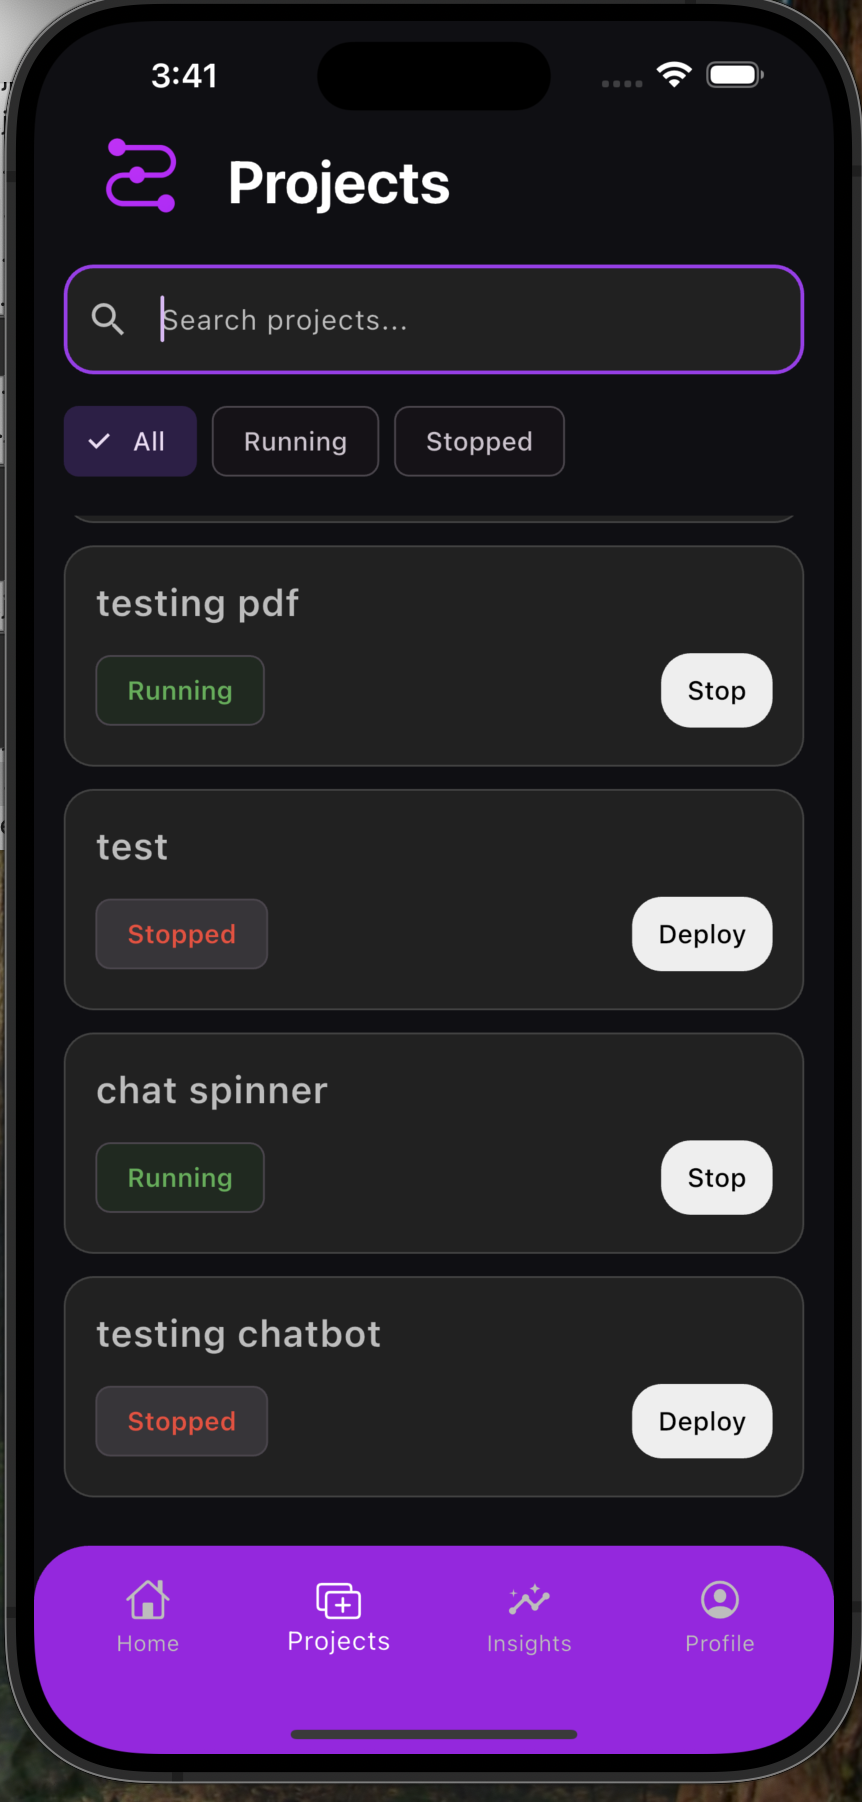
\includegraphics[width=0.42\textwidth]{images/mobile-app/admin-dashboard/project-page-D.png}
    \caption{Projects Screen}
    \label{fig:mobile-projects}
\end{figure}

\vspace{0.2cm}
\noindent\textbf{Main Components}

\begin{itemize}
    \item Search Bar
    \item Workflow Cards
    \item Status Indicators
    \item Deploy Button
    \item Stop Button
    \item Floating Action Button
\end{itemize}

\vspace{0.2cm}
\noindent\textbf{Behavior \& Logical Flows}

\begin{itemize}
    \item Retrieves the authenticated user's workflow projects using secured REST API requests.
    \item Displays project information in organized workflow cards.
    \item Allows users to search for workflow projects by name.
    \item Shows the current execution status of each workflow.
    \item Enables workflow deployment and termination directly from the project list.
\end{itemize}

%%%%%%%%%%%%%%%%%%%%%%%%%%%%%%%%%%%%%%%%%%%%%%%%%%%%%%%%%%%%

\subsubsection{Create Project}

\textbf{Purpose:}
Allows users to create a new workflow project directly from the mobile application.

\begin{figure}[H]
    \centering
    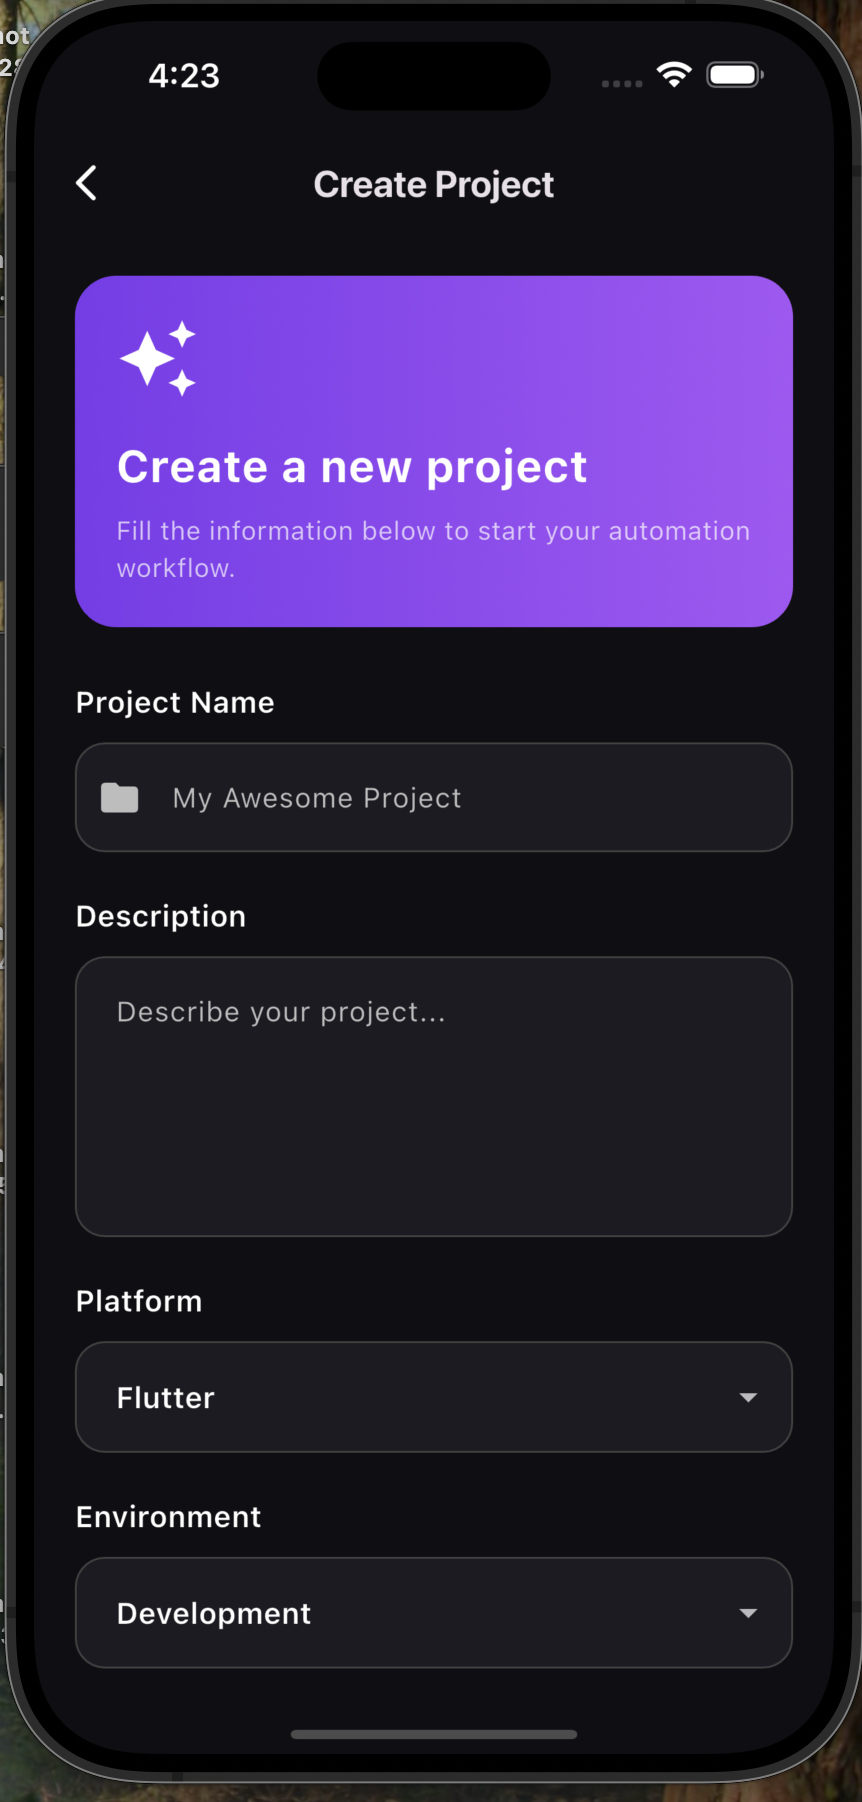
\includegraphics[width=0.40\textwidth]{images/mobile-app/admin-dashboard/create_project.png}
    \hfill
    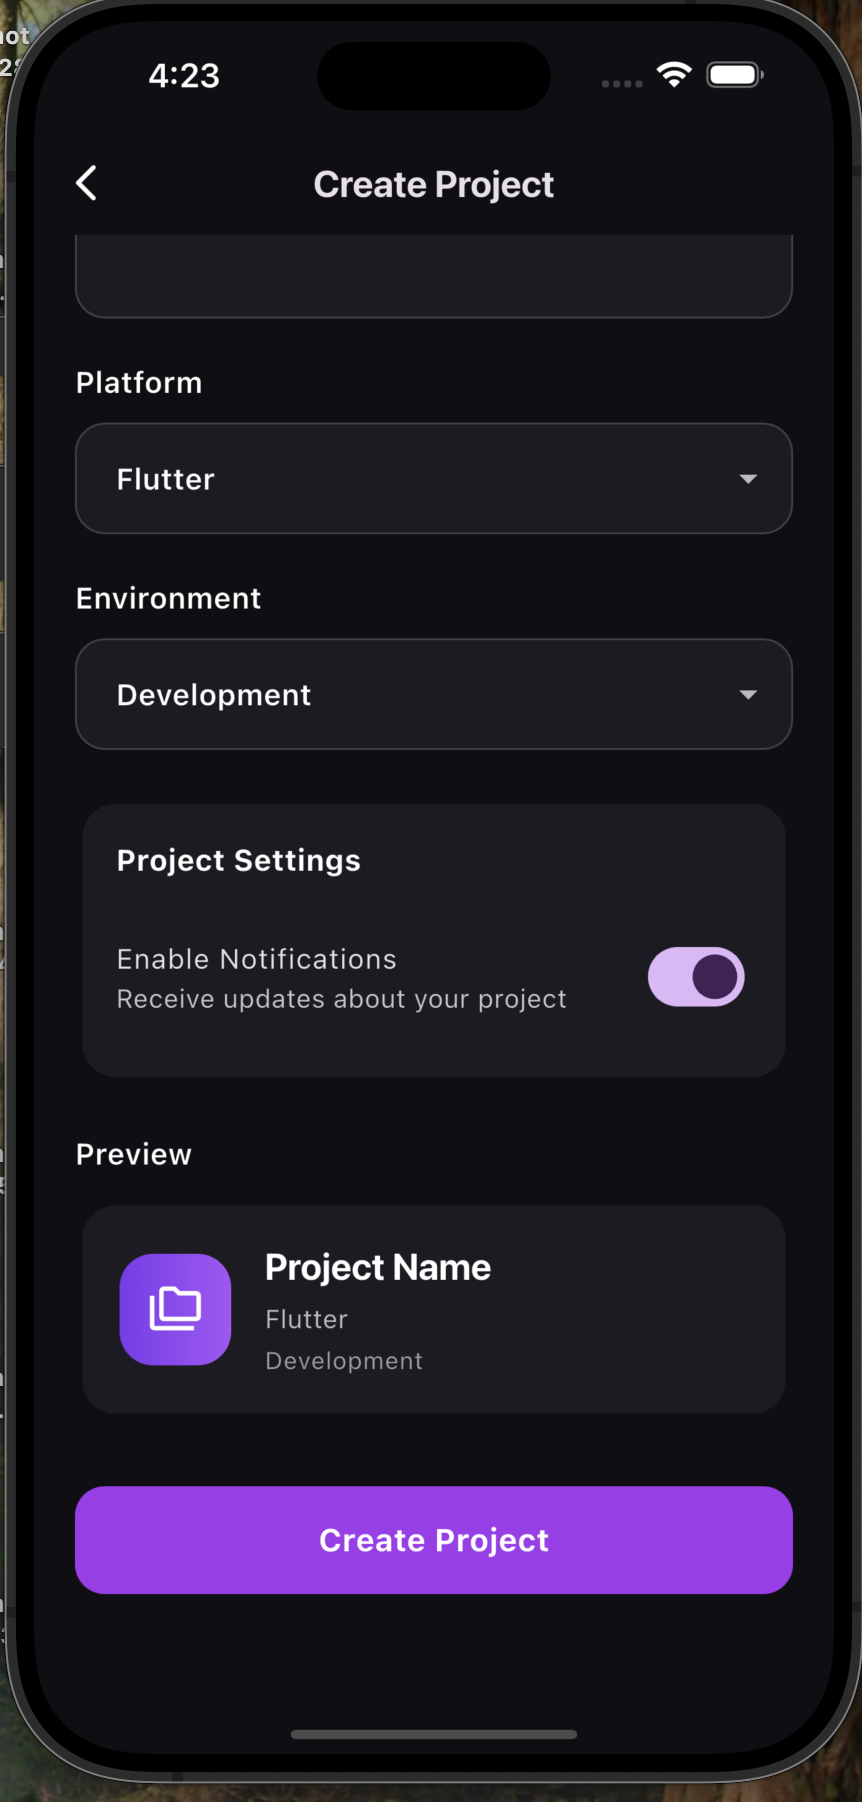
\includegraphics[width=0.40\textwidth]{images/mobile-app/admin-dashboard/create-project2D.png}
    \caption{Create Project}
    \label{fig:create-project}
\end{figure}

\vspace{0.2cm}
\noindent\textbf{Behavior \& Logical Flows}

\begin{itemize}
    \item Allows users to enter the required project information.
    \item Validates mandatory input fields before submitting the request.
    \item Sends the project creation request to the backend through authenticated REST APIs.
    \item Displays success or error feedback after the operation completes.
    \item Refreshes the project list automatically after successful project creation.
\end{itemize}

%%%%%%%%%%%%%%%%%%%%%%%%%%%%%%%%%%%%%%%%%%%%%%%%%%%%%%%%%%%%

\subsubsection{Import Workflow}

\textbf{Purpose:}
Allows users to import existing workflow configurations instead of creating them manually.

\begin{figure}[H]
    \centering
    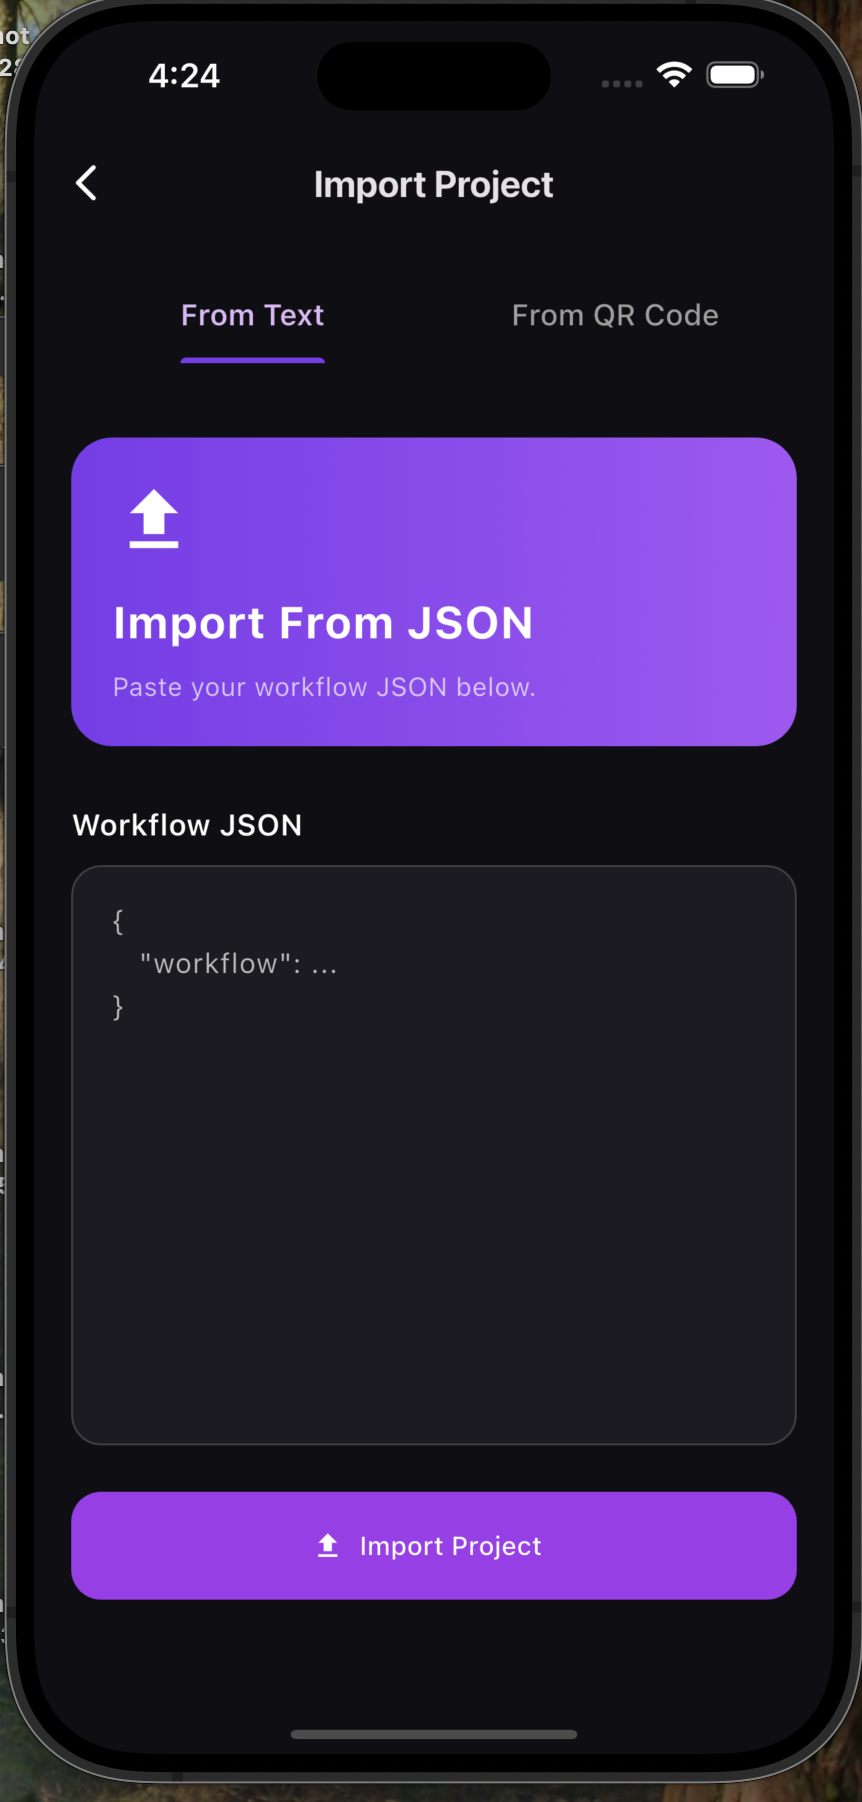
\includegraphics[width=0.40\textwidth]{images/mobile-app/admin-dashboard/import-page-json-D.png}
    \hfill
    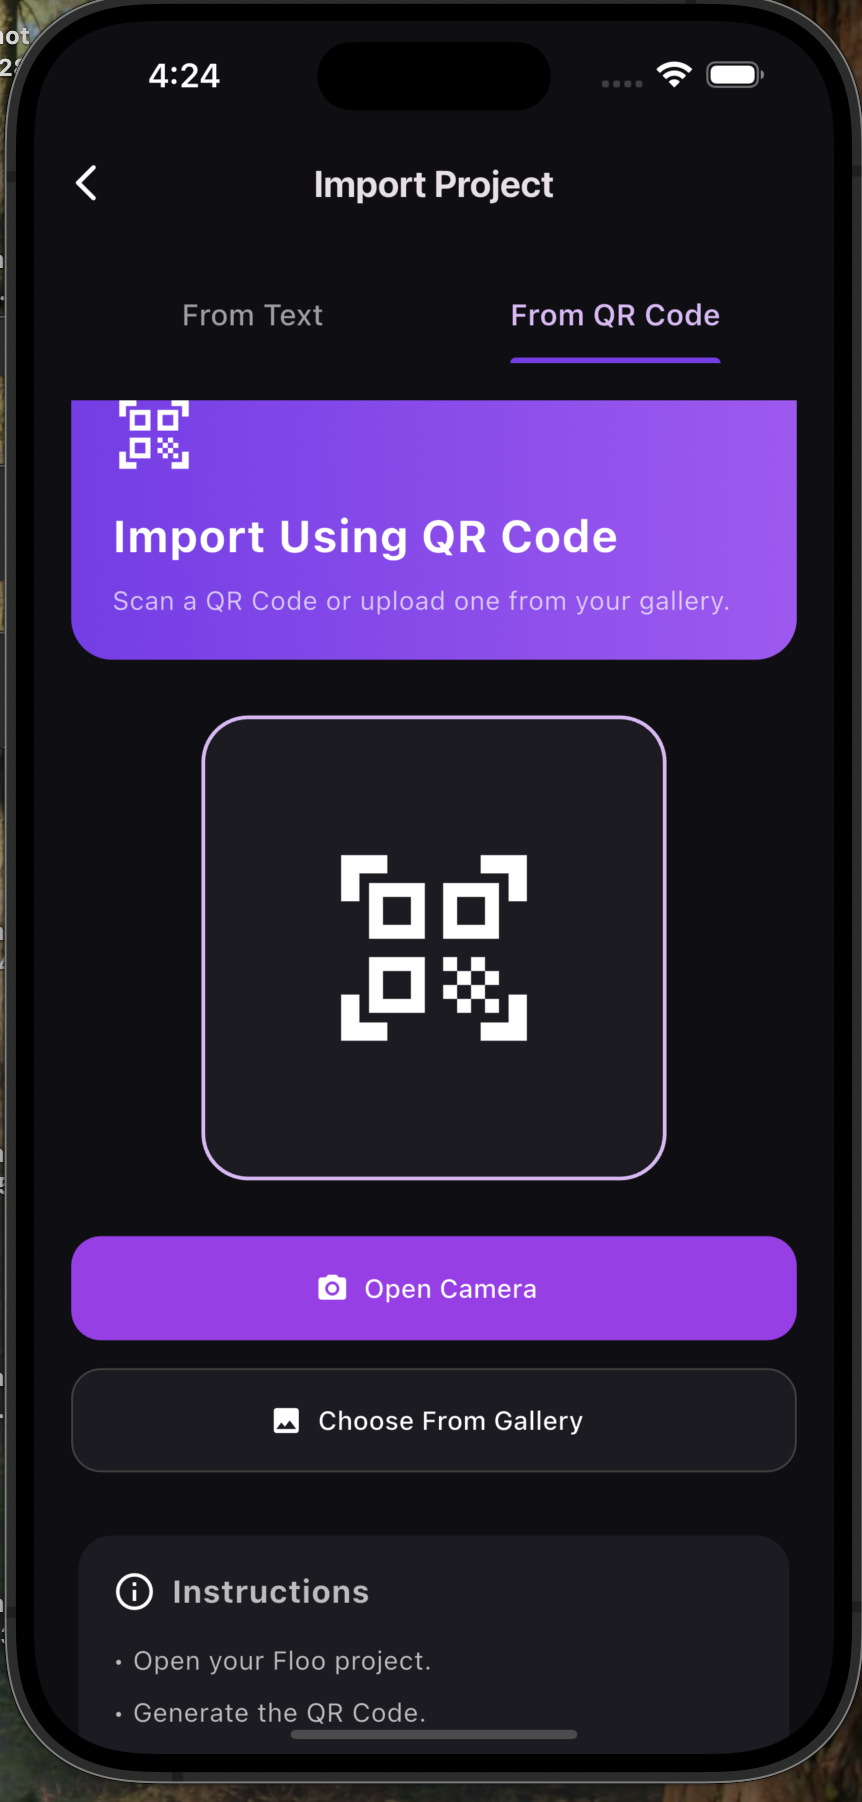
\includegraphics[width=0.40\textwidth]{images/mobile-app/admin-dashboard/import-page-qr-D.png}
    \caption{Import Workflow}
    \label{fig:import-workflow}
\end{figure}

\vspace{0.2cm}
\noindent\textbf{Supported Import Methods}

\begin{itemize}
    \item Import workflow using JSON files.
    \item Import workflow using QR codes.
\end{itemize}

\vspace{0.2cm}
\noindent\textbf{Behavior \& Logical Flows}

\begin{itemize}
    \item Allows users to choose their preferred import method.
    \item Uploads workflow configuration data to the backend.
    \item Validates imported workflow data before adding it to the user's workspace.
    \item Displays confirmation messages after successful workflow import.
\end{itemize}

%%%%%%%%%%%%%%%%%%%%%%%%%%%%%%%%%%%%%%%%%%%%%%%%%%%%%%%%%%%%

\subsubsection{Workflow Operations}

\textbf{Purpose:}
Provides users with direct control over workflow execution without requiring access to the web dashboard.

\vspace{0.2cm}
\noindent\textbf{Supported Operations}

\begin{itemize}
    \item Deploy Workflow
    \item Stop Workflow
    \item View Workflow Status
    \item Refresh Project List
\end{itemize}

\vspace{0.2cm}
\noindent\textbf{Behavior \& Logical Flows}

\begin{itemize}
    \item Sends workflow deployment and termination requests through authenticated REST APIs.
    \item Updates workflow execution status after receiving backend responses.
    \item Prevents duplicate requests while operations are in progress.
    \item Displays loading indicators during asynchronous operations.
    \item Refreshes project information automatically after successful workflow actions.
\end{itemize}

%%%%%%%%%%%%%%%%%%%%%%%%%%%%%%%%%%%%%%%%%%%%%%%%%%%%%%%%%%%%

\subsubsection{Project State Management}

\textbf{Purpose:}
Maintains synchronization between the mobile interface and backend services while providing a responsive user experience.

\vspace{0.2cm}
\noindent\textbf{Behavior \& Logical Flows}

\begin{itemize}
    \item Loads workflow projects during screen initialization.
    \item Updates the user interface immediately after successful backend responses.
    \item Handles loading, success, and error states during API communication.
    \item Preserves project information while navigating between application screens.
    \item Displays appropriate feedback whenever communication with the backend fails.
\end{itemize}